\documentclass[paper=letter,fontsize=11pt]{scrartcl} % KOMA-article class
\usepackage[english]{babel}
\usepackage[utf8x]{inputenc}
\usepackage[protrusion=true,expansion=true]{microtype}
\usepackage{amsmath,amsfonts,amsthm}     % Math packages
\usepackage{graphicx}                    % Enable pdflatex
\usepackage[svgnames]{xcolor}            % Colors by their 'svgnames'
\usepackage{geometry}
	%\textheight=700px                    % Saving trees ;-)
%\usepackage{url}
\usepackage[colorlinks=true,
linkcolor=blue,
urlcolor=blue]{hyperref}
\usepackage{float}
\usepackage{etaremune}
\usepackage{wrapfig}
\usepackage{framed,graphicx,xcolor}
\definecolor{shadecolor}{rgb}{0.85,0.85,1}

\usepackage{attachfile}

\frenchspacing              % Better looking spacings after periods
\pagestyle{empty}           % No pagenumbers/headers/footers

%\addtolength{\voffset}{-40pt}
%\addtolength{\textheight}{20pt}

\setlength\topmargin{0pt}
\addtolength\topmargin{-\headheight}
\addtolength\topmargin{-\headsep}
\setlength\oddsidemargin{0pt}
\setlength\textwidth{\paperwidth}
\addtolength\textwidth{-2in}
\setlength\textheight{\paperheight}
%\addtolength\textheight{-3in}
\addtolength\textheight{-2in}
\usepackage{layout}

%%% Custom sectioning}{sectsty package)
%%% ------------------------------------------------------------
\usepackage{sectsty}

\sectionfont{%			            % Change font of \section command
	\usefont{OT1}{phv}{b}{n}%		% bch-b-n: CharterBT-Bold font
	\sectionrule{0pt}{0pt}{-5pt}{3pt}}

%%% Macros
%%% ------------------------------------------------------------
\newlength{\spacebox}
\settowidth{\spacebox}{8888888888}			% Box to align text
\newcommand{\sepspace}{\vspace*{1em}}		% Vertical space macro

\newcommand{\MyName}[1]{ % Name
		\Huge \usefont{OT1}{phv}{b}{n} \hfill #1
		\par \normalsize \normalfont}

\newcommand{\MySlogan}[1]{ % Slogan}{optional)
		\large \usefont{OT1}{phv}{m}{n}\hfill \textit{#1}
		\par \normalsize \normalfont}

\newcommand{\NewPart}[2]{\section*{\uppercase{#1} #2}}

\newcommand{\PersonalEntry}[2]{
		\noindent\hangindent=2em\hangafter=0 % Indentation
		\parbox{\spacebox}{        % Box to align text
		\textit{#1}}		       % Entry name}{birth, address, etc.)
		\hspace{1.5em} #2 \par}    % Entry value

\newcommand{\SkillsEntry}[2]{      % Same as \PersonalEntry
		\noindent\hangindent=2em\hangafter=0 % Indentation
		\parbox{\spacebox}{        % Box to align text
		\textit{#1}}			   % Entry name}{birth, address, etc.)
		\hspace{1.5em} #2 \par}    % Entry value

\newcommand{\EducationEntry}[4]{
		\noindent \textbf{#1} \hfill      % Study
		\colorbox{White}{%
			\parbox{10em}{%
			\hfill\color{Black}#2}} \par  % Duration
		\noindent \textit{#3} \par        % School
		\noindent\hangindent=2em\hangafter=0 \small #4 % Description
		\normalsize \par}

\newcommand{\WorkEntry}[4]{				  % Same as \EducationEntry
		\noindent \textbf{#1} \hfill      % Jobname
		\colorbox{White}{\color{White}#2} \par  % Duration
		\noindent \textit{#3} \par              % Company
		\noindent\hangindent=2em\hangafter=0 \small #4 % Description
		\normalsize \par}

\newcommand{\PaperEntry}[7]{
		\noindent #1, ``\href{#7}{#2}", \textit{#3} \textbf{#4}, #5 (#6).}


\newcommand{\ArxivEntry}[3]{
		\noindent #1, ``\href{http://arxiv.org/abs/#3}{#2}", \textit{{cond-mat/}#3}.}

\newcommand{\BookEntry}[4]{
		\noindent #1, ``\href{#3}{#4}", \textit{#3}.}

\newcommand{\FundingEntry}[5]{
        \noindent #1, ``#2", \$#3 (#4, #5).}

\newcommand{\TalkEntry}[4]{
		\noindent #1, #2, #3 #4}

\newcommand{\ThesisEntry}[5]{
		\noindent #1 -- #2 #3 ``#4" \textit{#5}}

\newcommand{\CourseEntry}[3]{
		\noindent \item{#1: \textbf{#2} \\ #3}}

%%% Begin Document
%%% ------------------------------------------------------------
\begin{document}

%\layout

% you can upload a photo and include it here...
\begin{wrapfigure}{l}{0.5\textwidth}
	\vspace*{-2em}
		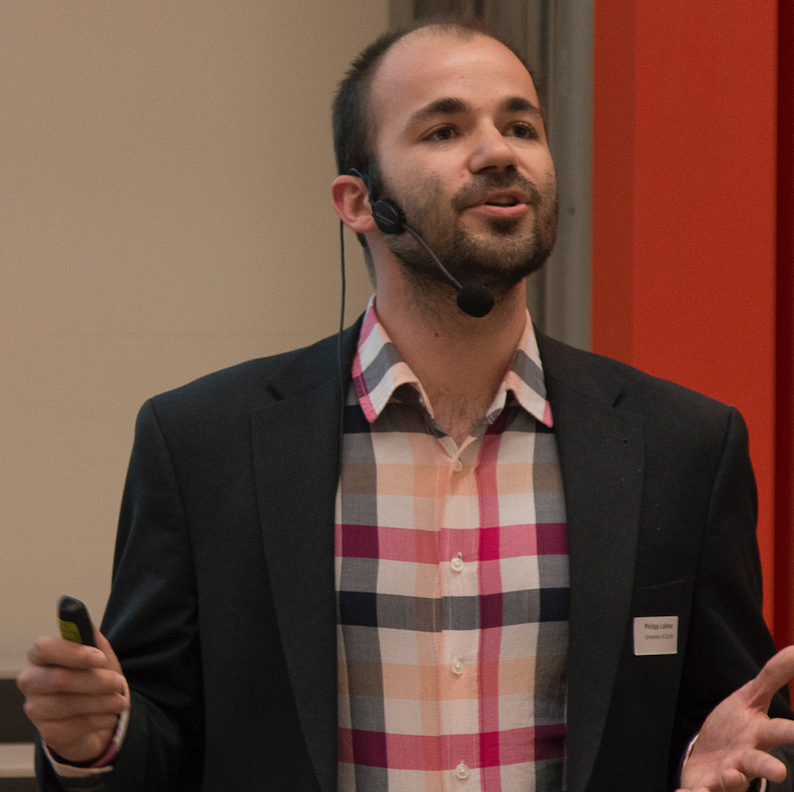
\includegraphics[width=0.18\textwidth]{profile.png}
\end{wrapfigure}

\MyName{Philipp Leitner}
\MySlogan{Teaching Activities (\today)}

\sepspace

\NewPart{Pedagogical Training}{}

\begin{itemize}
\item \textbf{Supervision of research} (2017, 2 ECTS)
\item \textbf{Undervisning och lärande på universitetsnivå}  (2017, 3 ECTS)
\item \textbf{Perspectives on learning}  (2018, 2.5 ECTS)
\item \textbf{Enhancing learning through writing} (2018, 5 ECTS)
\end{itemize}

\NewPart{Teaching Activities}{}

\subsection*{Teaching at Chalmers $|$ GU}
\begin{itemize}
	\item Mobile and Web Development (DIT341) (since 2019, $\approx$ 80 students)
  \item Data Management (DIT032/DAT335) (since 2018, $\approx$ 150 students)
\end{itemize}

\subsection*{Previous Teaching at University of Zurich}
\begin{itemize}
  \item Informatik 1 (fall 2014 -- 2016, $\approx$ 250 students)
  \item Advanced Software Engineering (spring 2014 -- 2017, 10 -- 20 students)
  \item Seminar Advanced Software Engineering (fall 2015 -- 2016, 10 -- 20 students)
  \item Master Basismodul (2014 -- 2017)
  \item Informatik-Vertiefung (2014 -- 2017)
\end{itemize}

\subsection*{Previous Teaching at TU Vienna}
\begin{itemize}
  \item VU 2.0 Advanced Internet Computing (fall 2008 - 2013, 140 students)
  \item VU 4.0 Distributed Systems Technologies (spring 2009 - 2013, 140 students)
  \item PR 4.0 Internet Computing Lab Work (spring 2009 - 2013)
  \item UE 2.0 Verteilte Systeme (fall 2009 - fall 2010, $\approx$ 400 students)
  \item VU 2.0 Grid Computing (spring 2008 - spring 2009, 10 students)
\end{itemize}

\subsection*{Thesis Supervision at Chalmers $|$ University of Gothenburg}

\begin{itemize}
	\item Elsada Lagumdzic: Evaluation of Open Source Function as a Service Frameworks: An Experimental Analysis of Auto Scaling Characteristics (bachelor thesis, 2020)
	\item Joel Sanderöd Roxell and and Matthias Lundell: Automatic container profiling
and resource prediction using container orchestration (master's thesis, 2019)
	\item Yunfang Guo: The Impact of Adopting Continuous Integration on the Delivery Time of Pull Requests - A Partial Replication and Extension (master's thesis, 2019)
	\item Joel Rollny: An Extensible Framework for Large-Scale Mining of Performance Microbenchmarks (master's thesis, 2018)
  \item Viktor Holmqvist and Jonathan Nilsfors: Cachematic - Automatic Invalidation in Application-Level Caching Systems (master's thesis, 2018)
\end{itemize}

\subsection*{Thesis Supervision at University of Zurich}

\emph{All co-supervised with Prof. Harald C. Gall.}

\begin{itemize}
  \item Michael Susplugas: Continuous Integration and Deployment -- Case Study in an Energy Trading Company (master's thesis, 2016)
	\item Christian Davatz: Application-aware Benchmarking of IaaS Cloud Services (master's thesis, 2016)
	\item Bj\"orn Hasselmann: Mining Performance-Relevant Code Changes from Source Code Repositories (bachelor thesis, 2016)
  \item Emanuel St\"ockli: Predicting the Costs of Code Changes in Microservice Architectures based on Runtime Feedback  (master's thesis, 2015)
  \item Ilia Rhyzhov: Performance Analysis of Virtual Machines from Two Major IaaS Providers -- Amazon Web Services (EC2) and Google Compute Engine (GCE)  (master's thesis, 2015)
  \item Christian Bosshard: Feedback Driven Development -- Bringing Runtime Metrics to the Developer  (master's thesis, 2015)
  \item Joel Scheuner: Cloud WorkBench - A Web-Based Framework for Benchmarking Public Cloud Services (bachelor thesis, 2014)
\end{itemize}

\subsection*{Master's Thesis Supervision at TU Vienna}

\emph{All co-supervised with Prof. Schahram Dustdar.}

\begin{itemize}
  \item Fritz Schrogl: Transparently Migrating Java Objects at Runtime in an Infrastructure-as-a-Service Cloud (2014)
  \item J\"urgen Cito: Statistical Methods in Web Performance (2014)
  \item Constantin-Claudiu Gavrilete: Exploiting User Behavior and Markup Structures to Improve Search Result Rankings (2013)
  \item Rene Nowak: Towards Providing Unified Access To Cloud Data Storage Services (2013)
  \item Denitsa Djamiykova: Monitoring the Correspondence of Physical and Virtual Network Resources in OpenFlow Based Software Defined Networks (2013)
  \item Johannes Ferner:  Using Time Series Analysis to Predict Service Level Agreement Violations in Service Compositions (2012)
\item Petra Bierleutgeb:  VRoxy -- Enriching SOAs With Proxy-Based Dynamic
  Binding and Reporting Based on VRESCo (joint work with mercatis information systems GmbH, 2012)
  \item Matthias Irlacher: Using Domain-specific Languages for Event-based QoS monitoring in Service-oriented Environments. (co-supervised with Ernst Oberortner, 2011)
  \item Mathias Hess:  Reducing SLA Violations of Composite Services Deployed to the Cloud (2011)
  \item Stefan Prennsch\"utz-Sch\"utzenau:  SOA Security Policy Validation and
  Authoring (work carried out at IBM T.J. Watson Research Center, New York, 2011)
    \item Anton Korosec:  Deploying a Web Service Runtime Environment into the
  Cloud (2010)
  \item Klaus Zettler:  Planung, Konzeption und Implementierung eines Virtual
  Campus im Rahmen von S-Cube (2010)
  \item Waldemar Hummer:  Towards a Domain-Specific Language for Defining
  Intra-Service Protocols of Stateful Web Services (2009)
\end{itemize}


\end{document}
